\chapter{Implementación}
\label{cap:implementacion}

Una de las partes más importantes de nuestro proyecto es el desarrollo del prototipo para una aplicación de explicaciones que haga uso de los diferentes conceptos que hemos estudiado en las fases iniciales del trabajo. En el capítulo anterior mostramos el proceso de diseño de su interfaz, así que ahora procederemos a detallar la parte de la implementación de la aplicación.\\

El código fuente de la aplicación está alojado en el siguiente repositorio de Github: \url{https://github.com/Adrigarr/TFG-2020-Code}. Sin embargo, para poder probar esta aplicación hay que usar este enlace: \url{https://explicaciones.herokuapp.com/}.\\


\section{Procesamiento y manejo de la muestra}

Partimos de una muestra (o \textbf{dataset}) de alrededor de 19 millones de líneas, obtenido a partir de la API de \textbf{Last.fm} \cite{lastfm}, una plataforma que almacena y proporciona mucho contenido musical. Constaba de los siguientes campos: \textbf{<user, timestamp, artist, song>}, los cuales hacen referencia al usuario que ha escuchado la canción, la fecha en la que fue escuchada, el nombre del artista y el título de la canción respectivamente.\\

El primer paso fue hacer un pequeño estudio del dataset para hacernos una idea de cómo era nuestra muestra y qué podríamos sacar de ella. Se trataba de un dataset con muy pocos campos que no daba información ninguna sobre la canción o el artista, sino que solo proporcionaba un medio para poder obtenerla de una fuente externa. Hicimos una limpieza del dataset, ya que había numerosos valores que eran nulos en determinados campos o no tenían una codificación correcta.\\

Es en este punto donde comenzamos a pensar cómo queríamos mostrar la información que podíamos ofrecer previa al funcionamiento de la aplicación. Dudábamos entre permitir utilizar cualquier objeto del dataset o restringirlo solo a algunos.\\

En la librería de Wikidata, por motivos obvios, se debe poner como entrada de cualquier función de búsqueda el código identificador del objeto sobre el que se quiere obtener información. Estos identificadores son fijos y únicos para cada uno de los objetos que están registrados en la página. Con nuestra librería somos capaces de, a partir de un string que represente un título de canción o un artista, género, etc., obtener su respectivo identificador para posteriormente procesar las consultas.\\

El problema aquí es que para obtener el identificador del objeto, su nombre o título debía ser exacto al que aparecía en Wikidata, pues de cualquier otra forma se lanzaría una excepción. Por ejemplo, intentar obtener el identificador de la canción ``Don’t Stop me Now'' sería incorrecto, porque en Wikidata figura como ``Don’t Stop Me Now''. Debido a esto, es necesario hacer un parseo previo de cualquier String (o cadena de caracteres) que se vaya a utilizar como entrada.\\

Finalmente decidimos crear una lista preseleccionada y parseada de las canciones más populares de todo el dataset. Para ello ordenamos las canciones del dataset por popularidad descendente, entendiendo como popularidad la cantidad de veces que aparecían en la muestra. Después elaboramos un script que recorría todas ellas, ejecutaba el parseo y finalmente comprobaba si era posible obtener los datos de Wikidata mediante una llamada a un método de la librería SPARQLWrapper que retornaba un objeto si se había encontrado información del artista o una excepción en caso contrario. Finalmente obtuvimos una lista con tuplas de canciones-artista con las que trabajar sabiendo que no íbamos a obtener fallos o excepciones(sin tener en cuenta la posible cantidad de datos que podríamos obtener de cada una de ellas).\\

Empezamos con un dataset de las 2500 canciones más populares y fuimos capaces de obtener la información de 1408 canciones con su determinado artista. Cabe señalar que en cada búsqueda de una canción se debe añadir su artista, pues hay varias canciones con el mismo título que no podrían diferenciarse de otro modo.\\

Nuestra aplicación final funciona con este dataset limitado pero que cuenta con la seguridad de que se pueden obtener datos fiables sin importar la canción que se elija. Además, al haber escogido las canciones con mayor popularidad nos vamos a encontrar con mayor cantidad de datos ya que estas eran las que más documentadas estaban. a diferencia de las que estaban en la parte inferior del dataset, que eran muy poco conocidas y apenas se podían sacar datos valiosos sobre ellas.


\section{Arquitectura de la aplicación}

Nuestra aplicación adopta una arquitectura cliente-servidor. En esta arquitectura, las tareas se reparten entre los proveedores de servicios, llamadas servidores, y los demandantes de esos servicios, llamados clientes. Por esto mismo, el servidor es el encargado de realizar todas las gestiones mientras que los clientes se limitan a hacer peticiones al servidor y recibir los resultados de esas gestiones \cite{reese2000}.\\

Además, en nuestro caso el servidor no almacena todos los datos y recursos necesarios para el funcionamiento de la aplicación. Para poder gestionar apropiadamente las peticiones de los clientes, nuestro servidor debe ponerse en contacto con Wikidata, de donde obtendrá la información vital a procesar para obtener los resultados que se envían posteriormente al cliente que haya hecho la petición. En la Figura~\ref{fig:diagramaCS} se ve una representación de nuestra arquitectura.\\

\begin{figure}[h!]
	\centering
	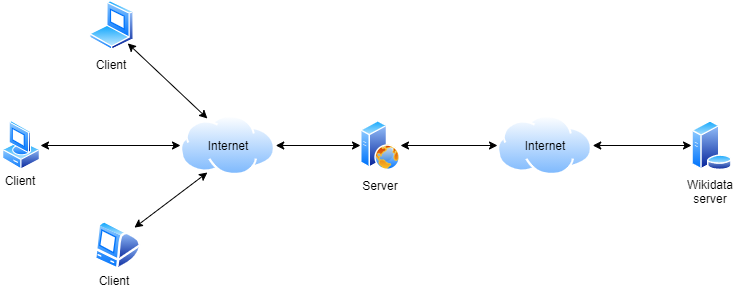
\includegraphics[width = 0.9\textwidth]{Imagenes/Bitmap/Diagrama cliente servidor.png}
	\caption{Diagrama de la arquitectura cliente-servidor de la aplicación}
	\label{fig:diagramaCS}
\end{figure}

Para explicar mejor su funcionamiento, estudiaremos cada una de las partes de la arquitectura por separado.\\

\subsection{Cliente}

El cliente es la parte con la que interactúan los usuarios de la aplicación. Como la nuestra es una aplicación web, el cliente es la parte del navegador y la interfaz visual que se muestra en el mismo.\\

En la interfaz se muestra la lista de canciones a elegir, la cual recibe desde el servidor mediante un archivo de formato CSV. Una vez el usuario escoja dos de esas canciones y confirme la selección, el cliente enviará una petición al servidor. El servidor realizará una serie de operaciones para comparar las canciones y obtener los grafos de explicaciones deseados.\\

Cuando el servidor haya completado su parte, devolverá al cliente un archivo de formato JavaScript donde están contenidas las estructuras de datos necesarias para dibujar los grafos. Empleando la librería vis.js, el cliente dibujará dos grafos y los mostrará por pantalla para que el usuario pueda verlos.\\

\subsection{Servidor}

El servidor es la parte que escucha las peticiones del cliente y hace las gestiones necesarias para devolverle la información deseada. Esta es la parte responsable de la mayoría de procesos existentes en nuestra aplicación, desde gestionar consultas a Wikidata hasta tratar los datos obtenidos para dibujar los grafos de explicaciones.\\

Para explicar el funcionamiento del servidor debemos repasar los módulos que lo conforman, cuya relación se puede observar en la Figura~\ref{fig:diagramaComponentes}.\\

\begin{figure}[h!]
	\centering
	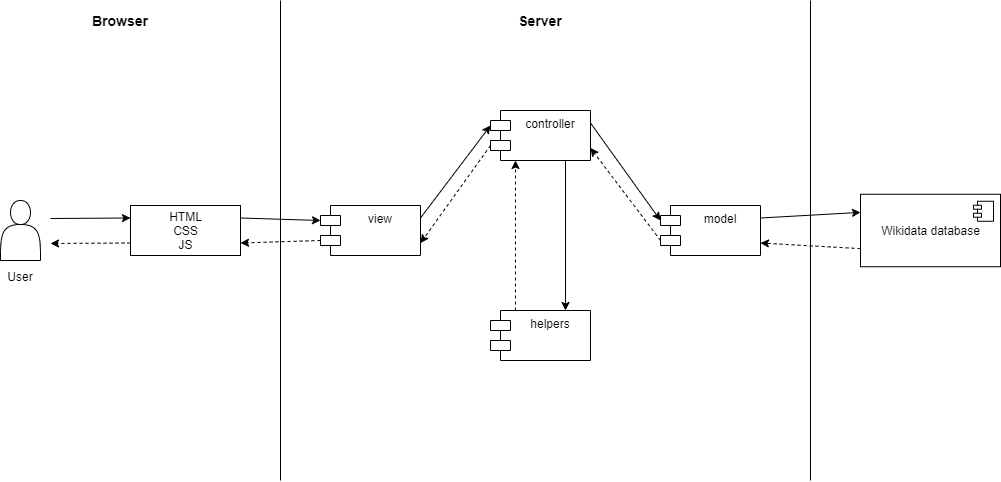
\includegraphics[width = 0.9\textwidth]{Imagenes/Bitmap/Diagrama componentes.png}
	\caption{Diagrama de componentes de la aplicación}
	\label{fig:diagramaComponentes}
\end{figure}

El módulo ``view'' contiene las plantillas de la interfaz, es decir, lo que verá el usuario por pantalla una vez se haya renderizado en el navegador.\\

El módulo ``controller'' es el centro de control entre el resto de módulos. Todas las comunicaciones entre módulos pasan por aquí. Recibe las peticiones de ``view'', que se originan por las elecciones del usuario, y a su vez pide al módulo ``model'' que gestione esa petición y devuelva los resultados. Con los resultados de ``model'', ``controller'' le pide al módulo ``helpers'' que procese esos datos para poder dibujar los grafos, tras lo cual ya está listo para devolver los resultados a ``view''.\\

El módulo ``model'' es uno de los más importantes. Se encarga de organizar los datos con los que se trabaja en la aplicación en clases, además de comunicarse con el servidor de Wikidata para obtener la información en la que se basan las explicaciones del sistema. Hace las consultas SPARQL y recoge los resultados en estructuras de datos con las que pueda trabajar el resto de la aplicación.\\

Por último, el módulo ``helpers'' es un módulo auxiliar para el dibujo de los grafos. Recibe los datos obtenidos de las consultas y los procesa para generar un archivo JavaScript que contiene las instrucciones necesarias para generar los grafos. Este será el que utilice el cliente para mostrar los grafos de explicaciones al usuario.\\

\subsection{Comunicación}

La comunicación con el servidor de Wikidata, se hace mediante el módulo ``model''. Este módulo se encarga de establecer la conexión con el punto de consultas de Wikidata para poder iniciar las consultas y recoger los datos devueltos. Como punto principal, encontramos la librería que nos ha permitido todas estas funciones SPARQLWrapper. Esta librería hace las funciones principales de establecer queries, crear un canal de conexión, y recibir en formato JSON, XML o CSV los datos obtenidos a partir de las mismas.\\

La conexión será establecida cada vez que el usuario quiera hacer una comparación entre un par de canciones, es decir el servidor hace una llamada por cada caso de uso que se quiera probar.\\

\begin{figure}[h!]
	\centering
	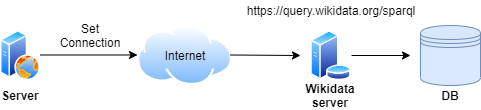
\includegraphics[width = 0.9\textwidth]{Imagenes/Bitmap/setConnection.png}
	\caption{Diagrama para establecer una conexión}
	\label{fig:diagramaConexion}
\end{figure}

\begin{figure}[h!]
	\centering
	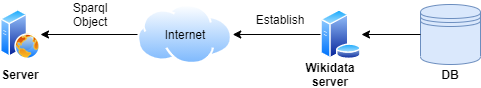
\includegraphics[width = 0.9\textwidth]{Imagenes/Bitmap/conexionReturn.png}
	\caption{Respuesta del servidor de Wikidata}
	\label{fig:respuestaWikidata}
\end{figure}

Una vez que obtengamos el objeto Sparql que devuelve el servidor de Wikidata ya podemos utilizarlo reiteradamente para poder mandar queries al servidor de Wikidata. Estas queries están predefinidas por las propiedades objeto de estudio y son las mismas para cada canción.\\

\begin{figure}[h!]
	\centering
	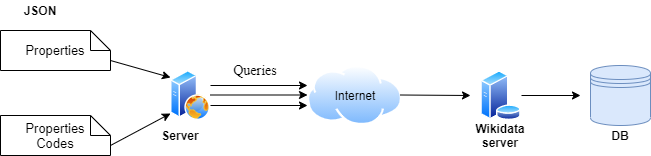
\includegraphics[width = 0.9\textwidth]{Imagenes/Bitmap/conexion.png}
	\caption{Lanzamiento de queries al servidor}
	\label{fig:queriesServidor}
\end{figure}


La entrada común para todo caso de uso en nuestro modelo de la aplicación para un determinado caso de uso, siempre es la misma: El par de canciones y el conjunto de propiedades que se va a estudiar sobre ellas para poder hallar las explicaciones. Esta información está guardada en formatos JSON y CSV, los cuáles al inicio del proceso, serán convertidos en diccionarios para poderlos procesar con las clases del modelo en Python.\\

Contamos con una jerarquía de clases, las cuales completan el módulo de conexión. Se encargarán de procesar las repuestas del servidor y crear progresivamente a medida que nos llegan respuestas varios documento que contengan todas las propiedades de cada canción y las relacione entre sí para poder obtener un grafo representable.\\

\section{Extensibilidad de la aplicación}

Se ha intentado dar un enfoque lo más aproximado posible a una estructura MVC~(Modelo-Vista-Controlador), con tal de poder hacer una aplicación lo más reutilizable posible y atenta a posibles cambios y modificaciones.\\

Para empezar, todas las propiedades y sus códigos para consultas están incluidas en diccionarios que son usados por el modelo. En un inicio creábamos queries con unos valores estáticos predeterminados pero nos dimos cuenta de que ese código no iba a poder ser reutilizable y era muy poco práctico. Poniendo un ejemplo, imaginemos que Wikidata implementa nuevas propiedades o nueva información en la base de datos de los artistas que añadir a nuestro estudio, contamos con métodos de adición con tan solo obtener el nombre y el código de esa nueva propiedad. El modelo no sufriría cambios en el código, ya que importa en cada lanzamiento todos estos diccionarios estáticos. De hecho, Wikidata es una base de datos que cambia constantemente por acción de diversos usuarios que completan y actualizan documentos constantemente, así que no es de extrañar que en cierto tiempo las explicaciones y por ende las propiedades activas, se queden obsoletas.\\

También como resultado final del modelo se proporciona un dataset en forma de archivos .json que contienen todas las relaciones con sus respectivos objetos y 4 datasets que representan información extra de las dos duplas canción/artista, de forma que son archivos estáticos y únicos en cada lanzamiento, nunca va a enviarse un número distinto de archivos.\\

En cuanto a la extensibilidad del DataSource de canciones y artistas, se trata de un módulo separado el cual utiliza como fuente el DataSet original de lastFM. El módulo se encarga de parsear los strings y procesarlo como hemos explicado en la sección de Preprocesamiento. No es una función que se pueda lanzar desde el main de la aplicación porque no está pensada para añadir canciones a voluntad por motivos de compatibilidad con la sintaxis y el manejo de Wikidata.\\

\section{Tecnologías y Herramientas utilizadas}
\label{sec:tecnologias}

Para la elaboración de este proyecto hemos tenido que estudiar numerosas tecnologías y herramientas diferentes. Algunas de ellas son viejas conocidas mientras que otras son completamente nuevas para nosotros y hemos tenido que familiarizarnos con ellas para poder trabajar con ellas.\\

A continuación haremos un repaso a las más relevantes para el desarrollo del proyecto, separándolas en distintos ámbitos para mayor comodidad.\\

\subsection{Programación}

\subsection*{Python}

Ha sido el lenguaje de programación principal, al menos en la parte del backend tanto para el núcleo del código que obtiene y relaciona los datos como para la creación de distintos scripts de ayuda, además de numerosas funciones para tratar los datos a representar en los grafos finales. Lo hemos escogido debido a su versatilidad y a su gran adaptación debido a la cantidad de librerías con las que cuenta.

\subsection*{Pandas y Numpy}

Dos librerías propias de Python, especializadas en el manejo y procesamiento de datos. Han sido de una utilidad vital ya que en gran parte del trabajo trabajamos con numerosos datasets y estas librerías nos proporcionan todo lo necesario para tratarlos, pudiendo así trabajar con ellos más fácilmente.

\subsection*{Sanic}

El framework seleccionado para desarrollar nuestra aplicación. Es un framework web asíncrono para Python cuyo objetivo es proporcionar una forma de crear un servidor que sea rápido y fácil de usar \cite{sanic}. Su sencillez para empezar a utilizarlo es uno de los principales factores que nos hizo decantarnos por él en lugar de otras opciones.

\subsection*{Jinja2}

Un motor de plantillas para Python basado en el sistema de plantillas de Django. Permite trabajar con documentos HTML con marcadores de posición que son llenados por lo que se le indica desde el código Python, permitiendo así utilizar variables en las vistas.\\

Esta función se utilizaba en una versión antigua de nuestro proyecto para tratar correctamente documentos cuyo título depende de la fecha y hora de su creación. Más adelante se cambió la forma en que se trataban estos documentos, pero seguimos utilizando Jinja2 para el formato de uso de las plantillas.

\subsection*{SPARQLWrapper}

Un wrapper para Python que permite ejecutar consultas SPARQL de forma remota \cite{sparqlwrapper}. Proporciona una funcionalidad esencial para nuestro trabajo, pues es lo que utilizamos para obtener la información de Wikidata desde nuestra aplicación.

\subsection*{HTML y CSS}

Dos lenguajes fundamentales para la programación web. Debido a la naturaleza de nuestra aplicación hemos recurrido a estos lenguajes para darle forma y estilo a la interfaz de explicaciones, aquella parte de nuestro proyecto con la que interactuarán los usuarios.

\subsection*{Javascript}

Al igual que los anteriores, este es un lenguaje de programación muy importante para el desarrollo web. Javascript es una parte integral de nuestro proyecto, pues es el lenguaje en el que se ha desarrollado la parte encargada de dibujar los grafos de explicaciones, además de otras funciones necesarias para el funcionamiento de la interfaz.

\subsection*{vis.js}

Esta es una librería de Javascript para visualización de datos  \cite{visjs}. Permite diversas representaciones gráficas, pero nosotros hemos empleado el componente Network para dibujar nuestros grafos de explicaciones. Es una librería bastante completa y con una documentación bien organizada, así que fue muy útil a la hora de plasmar en pantalla el resultado de nuestra investigación.

\subsection*{Jupyter-Notebooks}

Es un entorno informático interactivo basado en la web. Fue un entorno apropiado para realizar la prueba de scripts que nos ayudaron a limpiar y probar el dataset original.

\subsection{Organización}

\subsection*{Github}

Para poder almacenar y organizar todo el código en el que hemos trabajado conjuntamente. Nos ha permitido llevar un historial de versiones y actualizaciones de cada módulo del código. Github ha sido una herramienta apropiada no solo para llevar un control del código de la aplicación, sino también para la construcción de este mismo documento.

\subsection*{Google Drive}

Empleamos el servicio de alojamiento de archivos en la nube de Google para recoger y poner en común todos los documentos relacionados con la investigación previa al inicio del trabajo, además de para compartir recursos durante la realización del mismo. Su importancia quedó relegada a un segundo plano a medida que avanzaba el proyecto debido a que comenzamos a utilizar Github, pero cabe resaltar su utilidad durante las primeras fases.

\subsection*{Google Meet}

La aplicación de videoconferencias de Google fue una herramienta clave para mantener el contacto tanto con los directores del TFG como entre los miembros del equipo. Cuando las reuniones presenciales dejaron de ser posibles por motivos ajenos a nuestro control, se hizo necesario el uso de un servicio como este.

\subsection{Memoria}

\subsection*{LaTeX}

Este ha sido el procesador de textos elegido para la realización de este documento: la Memoria del TFG. Nos decantamos por este en lugar de otros procesadores como Word debido a las muchas posibilidades que tiene para generar documentos de calidad. Puntos como la estructura de capítulos, la estandarización de títulos o la forma de mostrar figuras (tanto imágenes como fragmentos de código), han hecho que nos resulte más sencilla la tarea de desarrollar esta memoria.

\subsection*{TeXiS}

TeXiS es una plantilla de \LaTeX para Tesis, Trabajos de Fin de Máster y otros documentos desarrollada por Marco Antonio y Pedro Pablo Gómez Martín. Es la plantilla que se ha usado como base para construir este documento y ha resultado de gran ayuda tanto para cuestiones de organización como para aprender a usar varias funcionalidades de \LaTeX, lo cual ha sido muy importante debido a nuestra falta de experiencia previa a este proyecto.

\subsection{Tecnologías y herramientas descartadas}

\subsection*{RDFstarTools}

Esta es una colección de librerías Java y herramientas de línea de comandos para procesar datos RDF* y consultas SPARQL* \cite{rdfstartools}. Proporciona varias funcionalidades, pero la verdaderamente relevante para nuestro proyecto es SPARQL* Parser, que sirve para hacer consultas SPARQL. Este parser está implementado sobre el framework Apache Jena.\\


Esta fue una de las opciones que barajamos para hacer consultas SPARQL desde nuestro código, pero acabamos decidiendo usar SPARQLWrapper en su lugar debido a que RDFstarTools es una colección de librerías de las cuales solo nos haría falta una pequeña parte. Tomando en consideración ambas opciones, nos pareció más adecuado utilizar Python junto con SPARQLWrapper debido ya que era más conciso y sencillo de implementar.

\subsection*{Java}

Uno de los lenguajes de programación de programación más extendidos y populares, especializado en la programación orientada a objetos. Al principio del proyecto nos planteamos utilizarlo como lenguaje principal para el backend de nuestra aplicación, sin embargo finalmente nos decantamos por Python.\\

Como ya hemos comentado antes, al decidir usar SPARQLWrapper para nuestras consultas SPARQL en lugar de RDFstarTools también nos pareció más adecuado descartar Java en favor de Python, aunque ambos habrían sido elecciones viables. 

\subsection*{Alchemy.js}

Alchemy.js es una aplicación de visualización de grafos para la web \cite{alchemyjs}. Está escrita en JavaScript con la librería D3.js como base y ofrece una manera sencilla y rápida de generar grafos. La mayoría de su personalización se lleva a cabo sobrescribiendo sus configuraciones por defecto, por lo que no requiere apenas implementar código JavaScript adicional.\\

Fue la primera opción contemplada para representar los grafos de nuestro proyecto debido a su sencillez de manejo y a su uso de archivos JSON para aportar los datos, algo que resultaba atractivo en un principio. Tras trabajar con ella durante un tiempo fue necesario descartarla por ciertas limitaciones a la hora de personalizar la representación según nuestro diseño, además de la falta de soporte por tratarse de un proyecto actualmente abandonado.
